\documentclass[]{article}
\usepackage{lmodern}
\usepackage{amssymb,amsmath}
\usepackage{ifxetex,ifluatex}
\usepackage{fixltx2e} % provides \textsubscript
\ifnum 0\ifxetex 1\fi\ifluatex 1\fi=0 % if pdftex
  \usepackage[T1]{fontenc}
  \usepackage[utf8]{inputenc}
\else % if luatex or xelatex
  \ifxetex
    \usepackage{mathspec}
  \else
    \usepackage{fontspec}
  \fi
  \defaultfontfeatures{Ligatures=TeX,Scale=MatchLowercase}
\fi
% use upquote if available, for straight quotes in verbatim environments
\IfFileExists{upquote.sty}{\usepackage{upquote}}{}
% use microtype if available
\IfFileExists{microtype.sty}{%
\usepackage{microtype}
\UseMicrotypeSet[protrusion]{basicmath} % disable protrusion for tt fonts
}{}
\usepackage[margin=1in]{geometry}
\usepackage{hyperref}
\hypersetup{unicode=true,
            pdftitle={evolutionary\_analysis},
            pdfauthor={Sahil Shah},
            pdfborder={0 0 0},
            breaklinks=true}
\urlstyle{same}  % don't use monospace font for urls
\usepackage{color}
\usepackage{fancyvrb}
\newcommand{\VerbBar}{|}
\newcommand{\VERB}{\Verb[commandchars=\\\{\}]}
\DefineVerbatimEnvironment{Highlighting}{Verbatim}{commandchars=\\\{\}}
% Add ',fontsize=\small' for more characters per line
\usepackage{framed}
\definecolor{shadecolor}{RGB}{248,248,248}
\newenvironment{Shaded}{\begin{snugshade}}{\end{snugshade}}
\newcommand{\AlertTok}[1]{\textcolor[rgb]{0.94,0.16,0.16}{#1}}
\newcommand{\AnnotationTok}[1]{\textcolor[rgb]{0.56,0.35,0.01}{\textbf{\textit{#1}}}}
\newcommand{\AttributeTok}[1]{\textcolor[rgb]{0.77,0.63,0.00}{#1}}
\newcommand{\BaseNTok}[1]{\textcolor[rgb]{0.00,0.00,0.81}{#1}}
\newcommand{\BuiltInTok}[1]{#1}
\newcommand{\CharTok}[1]{\textcolor[rgb]{0.31,0.60,0.02}{#1}}
\newcommand{\CommentTok}[1]{\textcolor[rgb]{0.56,0.35,0.01}{\textit{#1}}}
\newcommand{\CommentVarTok}[1]{\textcolor[rgb]{0.56,0.35,0.01}{\textbf{\textit{#1}}}}
\newcommand{\ConstantTok}[1]{\textcolor[rgb]{0.00,0.00,0.00}{#1}}
\newcommand{\ControlFlowTok}[1]{\textcolor[rgb]{0.13,0.29,0.53}{\textbf{#1}}}
\newcommand{\DataTypeTok}[1]{\textcolor[rgb]{0.13,0.29,0.53}{#1}}
\newcommand{\DecValTok}[1]{\textcolor[rgb]{0.00,0.00,0.81}{#1}}
\newcommand{\DocumentationTok}[1]{\textcolor[rgb]{0.56,0.35,0.01}{\textbf{\textit{#1}}}}
\newcommand{\ErrorTok}[1]{\textcolor[rgb]{0.64,0.00,0.00}{\textbf{#1}}}
\newcommand{\ExtensionTok}[1]{#1}
\newcommand{\FloatTok}[1]{\textcolor[rgb]{0.00,0.00,0.81}{#1}}
\newcommand{\FunctionTok}[1]{\textcolor[rgb]{0.00,0.00,0.00}{#1}}
\newcommand{\ImportTok}[1]{#1}
\newcommand{\InformationTok}[1]{\textcolor[rgb]{0.56,0.35,0.01}{\textbf{\textit{#1}}}}
\newcommand{\KeywordTok}[1]{\textcolor[rgb]{0.13,0.29,0.53}{\textbf{#1}}}
\newcommand{\NormalTok}[1]{#1}
\newcommand{\OperatorTok}[1]{\textcolor[rgb]{0.81,0.36,0.00}{\textbf{#1}}}
\newcommand{\OtherTok}[1]{\textcolor[rgb]{0.56,0.35,0.01}{#1}}
\newcommand{\PreprocessorTok}[1]{\textcolor[rgb]{0.56,0.35,0.01}{\textit{#1}}}
\newcommand{\RegionMarkerTok}[1]{#1}
\newcommand{\SpecialCharTok}[1]{\textcolor[rgb]{0.00,0.00,0.00}{#1}}
\newcommand{\SpecialStringTok}[1]{\textcolor[rgb]{0.31,0.60,0.02}{#1}}
\newcommand{\StringTok}[1]{\textcolor[rgb]{0.31,0.60,0.02}{#1}}
\newcommand{\VariableTok}[1]{\textcolor[rgb]{0.00,0.00,0.00}{#1}}
\newcommand{\VerbatimStringTok}[1]{\textcolor[rgb]{0.31,0.60,0.02}{#1}}
\newcommand{\WarningTok}[1]{\textcolor[rgb]{0.56,0.35,0.01}{\textbf{\textit{#1}}}}
\usepackage{graphicx,grffile}
\makeatletter
\def\maxwidth{\ifdim\Gin@nat@width>\linewidth\linewidth\else\Gin@nat@width\fi}
\def\maxheight{\ifdim\Gin@nat@height>\textheight\textheight\else\Gin@nat@height\fi}
\makeatother
% Scale images if necessary, so that they will not overflow the page
% margins by default, and it is still possible to overwrite the defaults
% using explicit options in \includegraphics[width, height, ...]{}
\setkeys{Gin}{width=\maxwidth,height=\maxheight,keepaspectratio}
\IfFileExists{parskip.sty}{%
\usepackage{parskip}
}{% else
\setlength{\parindent}{0pt}
\setlength{\parskip}{6pt plus 2pt minus 1pt}
}
\setlength{\emergencystretch}{3em}  % prevent overfull lines
\providecommand{\tightlist}{%
  \setlength{\itemsep}{0pt}\setlength{\parskip}{0pt}}
\setcounter{secnumdepth}{0}
% Redefines (sub)paragraphs to behave more like sections
\ifx\paragraph\undefined\else
\let\oldparagraph\paragraph
\renewcommand{\paragraph}[1]{\oldparagraph{#1}\mbox{}}
\fi
\ifx\subparagraph\undefined\else
\let\oldsubparagraph\subparagraph
\renewcommand{\subparagraph}[1]{\oldsubparagraph{#1}\mbox{}}
\fi

%%% Use protect on footnotes to avoid problems with footnotes in titles
\let\rmarkdownfootnote\footnote%
\def\footnote{\protect\rmarkdownfootnote}

%%% Change title format to be more compact
\usepackage{titling}

% Create subtitle command for use in maketitle
\providecommand{\subtitle}[1]{
  \posttitle{
    \begin{center}\large#1\end{center}
    }
}

\setlength{\droptitle}{-2em}

  \title{evolutionary\_analysis}
    \pretitle{\vspace{\droptitle}\centering\huge}
  \posttitle{\par}
    \author{Sahil Shah}
    \preauthor{\centering\large\emph}
  \postauthor{\par}
      \predate{\centering\large\emph}
  \postdate{\par}
    \date{7/2/2019}


\begin{document}
\maketitle

Saves sum of squares data

\hypertarget{r-markdown}{%
\subsection{R Markdown}\label{r-markdown}}

Generational Analysis of Mutations

\begin{Shaded}
\begin{Highlighting}[]
\KeywordTok{library}\NormalTok{(cowplot)}
\KeywordTok{library}\NormalTok{(dplyr)}
\KeywordTok{library}\NormalTok{(gridExtra)}
\KeywordTok{library}\NormalTok{(ggplot2)}
\KeywordTok{library}\NormalTok{(gtools)}

\KeywordTok{setwd}\NormalTok{(}\StringTok{"/home/wilkelab/pinetree-toys/three_genes_evolution/"}\NormalTok{)}

\NormalTok{best_file <-}\StringTok{ }\KeywordTok{list.files}\NormalTok{(}\StringTok{"/home/wilkelab/pinetree-toys/three_genes_evolution/"}\NormalTok{, }\DataTypeTok{pattern=}\StringTok{"best_replicated_gen_"}\NormalTok{)}
\NormalTok{best_file <-}\StringTok{ }\KeywordTok{mixedsort}\NormalTok{(}\KeywordTok{sort}\NormalTok{(best_file))}

\NormalTok{original_data <-}\StringTok{ }\KeywordTok{read.table}\NormalTok{(}\StringTok{"three_genes_test_file.tsv"}\NormalTok{, }\DataTypeTok{header=}\OtherTok{TRUE}\NormalTok{)}
\NormalTok{original_data <-}\StringTok{ }\KeywordTok{filter}\NormalTok{(original_data, species }\OperatorTok{==}\StringTok{ "proteinX"} \OperatorTok{|}\StringTok{ }\NormalTok{species }\OperatorTok{==}\StringTok{ "proteinY"} \OperatorTok{|}\StringTok{ }\NormalTok{species }\OperatorTok{==}\StringTok{ "proteinZ"}\NormalTok{)}
\NormalTok{original_line_plot <-}\StringTok{  }\KeywordTok{ggplot}\NormalTok{(original_data, }\KeywordTok{aes}\NormalTok{(}\DataTypeTok{fill=}\NormalTok{species, }\DataTypeTok{color=}\NormalTok{species, }\DataTypeTok{x=}\NormalTok{time, }\DataTypeTok{y=}\NormalTok{transcript)) }\OperatorTok{+}\StringTok{ }\KeywordTok{geom_line}\NormalTok{(}\DataTypeTok{stat=}\StringTok{"identity"}\NormalTok{) }\OperatorTok{+}\StringTok{ }\KeywordTok{ggtitle}\NormalTok{(}\StringTok{"Original Genome Function"}\NormalTok{)}

\NormalTok{gen0_data <-}\StringTok{ }\KeywordTok{read.table}\NormalTok{(}\StringTok{"gen_0_data.tsv"}\NormalTok{, }\DataTypeTok{header=}\OtherTok{TRUE}\NormalTok{)}
\NormalTok{gen0_data <-}\StringTok{ }\KeywordTok{filter}\NormalTok{(gen0_data, species }\OperatorTok{==}\StringTok{ "proteinX"} \OperatorTok{|}\StringTok{ }\NormalTok{species }\OperatorTok{==}\StringTok{ "proteinY"} \OperatorTok{|}\StringTok{ }\NormalTok{species }\OperatorTok{==}\StringTok{ "proteinZ"}\NormalTok{)}
\NormalTok{gen0_line_plot <-}\StringTok{  }\KeywordTok{ggplot}\NormalTok{(gen0_data, }\KeywordTok{aes}\NormalTok{(}\DataTypeTok{fill=}\NormalTok{species, }\DataTypeTok{color=}\NormalTok{species, }\DataTypeTok{x=}\NormalTok{time, }\DataTypeTok{y=}\NormalTok{transcript)) }\OperatorTok{+}\StringTok{ }\KeywordTok{geom_line}\NormalTok{(}\DataTypeTok{stat=}\StringTok{"identity"}\NormalTok{) }\OperatorTok{+}\StringTok{ }\KeywordTok{ggtitle}\NormalTok{(}\StringTok{"Genome Function at Generation 0"}\NormalTok{)}
  
\NormalTok{gen500_data <-}\StringTok{ }\KeywordTok{read.table}\NormalTok{(}\StringTok{"gen_500_data.tsv"}\NormalTok{, }\DataTypeTok{header=}\OtherTok{TRUE}\NormalTok{)}
\NormalTok{gen500_data <-}\StringTok{ }\KeywordTok{filter}\NormalTok{(gen500_data, species }\OperatorTok{==}\StringTok{ "proteinX"} \OperatorTok{|}\StringTok{ }\NormalTok{species }\OperatorTok{==}\StringTok{ "proteinY"} \OperatorTok{|}\StringTok{ }\NormalTok{species }\OperatorTok{==}\StringTok{ "proteinZ"}\NormalTok{)}
\NormalTok{gen500_line_plot <-}\StringTok{  }\KeywordTok{ggplot}\NormalTok{(gen500_data, }\KeywordTok{aes}\NormalTok{(}\DataTypeTok{fill=}\NormalTok{species, }\DataTypeTok{color=}\NormalTok{species, }\DataTypeTok{x=}\NormalTok{time, }\DataTypeTok{y=}\NormalTok{transcript)) }\OperatorTok{+}\StringTok{ }\KeywordTok{geom_line}\NormalTok{(}\DataTypeTok{stat=}\StringTok{"identity"}\NormalTok{) }\OperatorTok{+}\StringTok{ }\KeywordTok{ggtitle}\NormalTok{(}\StringTok{"Genome Function at Generation 500"}\NormalTok{)}

\NormalTok{gen1000_data <-}\StringTok{ }\KeywordTok{read.table}\NormalTok{(}\StringTok{"gen_1000_data.tsv"}\NormalTok{, }\DataTypeTok{header=}\OtherTok{TRUE}\NormalTok{)}
\NormalTok{gen1000_data <-}\StringTok{ }\KeywordTok{filter}\NormalTok{(gen1000_data, species }\OperatorTok{==}\StringTok{ "proteinX"} \OperatorTok{|}\StringTok{ }\NormalTok{species }\OperatorTok{==}\StringTok{ "proteinY"} \OperatorTok{|}\StringTok{ }\NormalTok{species }\OperatorTok{==}\StringTok{ "proteinZ"}\NormalTok{)}
\NormalTok{gen1000_line_plot <-}\StringTok{  }\KeywordTok{ggplot}\NormalTok{(gen1000_data, }\KeywordTok{aes}\NormalTok{(}\DataTypeTok{fill=}\NormalTok{species, }\DataTypeTok{color=}\NormalTok{species, }\DataTypeTok{x=}\NormalTok{time, }\DataTypeTok{y=}\NormalTok{transcript)) }\OperatorTok{+}\StringTok{ }\KeywordTok{geom_line}\NormalTok{(}\DataTypeTok{stat=}\StringTok{"identity"}\NormalTok{) }\OperatorTok{+}\StringTok{ }\KeywordTok{ggtitle}\NormalTok{(}\StringTok{"Genome Function at Generation 1000"}\NormalTok{)}

\NormalTok{final_data <-}\StringTok{ }\KeywordTok{last}\NormalTok{(best_file)}
\NormalTok{gen_final1_data <-}\StringTok{ }\KeywordTok{read.table}\NormalTok{(final_data, }\DataTypeTok{header=}\OtherTok{TRUE}\NormalTok{)}
\NormalTok{gen_final1_data <-}\StringTok{ }\KeywordTok{filter}\NormalTok{(gen_final1_data, species }\OperatorTok{==}\StringTok{ "proteinX"} \OperatorTok{|}\StringTok{ }\NormalTok{species }\OperatorTok{==}\StringTok{ "proteinY"} \OperatorTok{|}\StringTok{ }\NormalTok{species }\OperatorTok{==}\StringTok{ "proteinZ"}\NormalTok{)}
\NormalTok{gen_final1_line_plot <-}\StringTok{  }\KeywordTok{ggplot}\NormalTok{(gen_final1_data, }\KeywordTok{aes}\NormalTok{(}\DataTypeTok{fill=}\NormalTok{species, }\DataTypeTok{color=}\NormalTok{species, }\DataTypeTok{x=}\NormalTok{time, }\DataTypeTok{y=}\NormalTok{transcript)) }\OperatorTok{+}\StringTok{ }\KeywordTok{geom_line}\NormalTok{(}\DataTypeTok{stat=}\StringTok{"identity"}\NormalTok{) }\OperatorTok{+}\StringTok{ }\KeywordTok{ggtitle}\NormalTok{(}\StringTok{"Genome Function of Best Genome Found"}\NormalTok{)}

\NormalTok{gen_plots <-}\StringTok{ }\KeywordTok{grid.arrange}\NormalTok{(original_line_plot, gen0_line_plot, gen500_line_plot, gen1000_line_plot, gen_final1_line_plot, }\DataTypeTok{nrow=}\DecValTok{2}\NormalTok{, }\DataTypeTok{ncol=}\DecValTok{3}\NormalTok{, }\DataTypeTok{top=}\StringTok{"Generational Pattern of Gene Transcripts"}\NormalTok{)}
\end{Highlighting}
\end{Shaded}

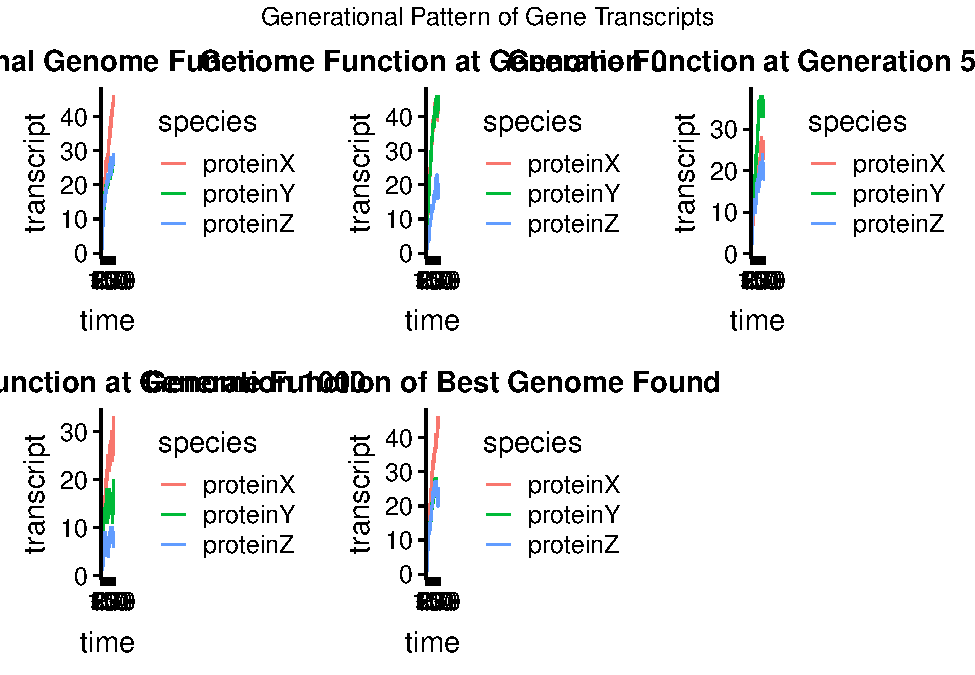
\includegraphics{evolutionary_analysis_files/figure-latex/cars-1.pdf}

\begin{Shaded}
\begin{Highlighting}[]
\KeywordTok{ggsave}\NormalTok{(}\StringTok{"/home/wilkelab/pinetree-toys/three_genes_evolution/gen_graphs.pdf"}\NormalTok{, gen_plots, }\DataTypeTok{width=}\DecValTok{20}\NormalTok{, }\DataTypeTok{height=}\DecValTok{10}\NormalTok{)}
\end{Highlighting}
\end{Shaded}

Evolutionary Analysis of Mutations

\begin{verbatim}
## Warning in plots_list[i] <- plot_name: number of items to replace is not a
## multiple of replacement length

## Warning in plots_list[i] <- plot_name: number of items to replace is not a
## multiple of replacement length

## Warning in plots_list[i] <- plot_name: number of items to replace is not a
## multiple of replacement length

## Warning in plots_list[i] <- plot_name: number of items to replace is not a
## multiple of replacement length

## Warning in plots_list[i] <- plot_name: number of items to replace is not a
## multiple of replacement length

## Warning in plots_list[i] <- plot_name: number of items to replace is not a
## multiple of replacement length

## Warning in plots_list[i] <- plot_name: number of items to replace is not a
## multiple of replacement length

## Warning in plots_list[i] <- plot_name: number of items to replace is not a
## multiple of replacement length

## Warning in plots_list[i] <- plot_name: number of items to replace is not a
## multiple of replacement length

## Warning in plots_list[i] <- plot_name: number of items to replace is not a
## multiple of replacement length

## Warning in plots_list[i] <- plot_name: number of items to replace is not a
## multiple of replacement length

## Warning in plots_list[i] <- plot_name: number of items to replace is not a
## multiple of replacement length

## Warning in plots_list[i] <- plot_name: number of items to replace is not a
## multiple of replacement length

## Warning in plots_list[i] <- plot_name: number of items to replace is not a
## multiple of replacement length

## Warning in plots_list[i] <- plot_name: number of items to replace is not a
## multiple of replacement length
\end{verbatim}

\includegraphics{evolutionary_analysis_files/figure-latex/pressure-1.pdf}

Note that the \texttt{echo\ =\ FALSE} parameter was added to the code
chunk to prevent printing of the R code that generated the plot.


\end{document}
